%\documentclass[border=3mm]{standalone}
%\usepackage{pgfplots}
%\pgfplotsset{compat=newest}
%\pagestyle{empty}
%\begin{document}
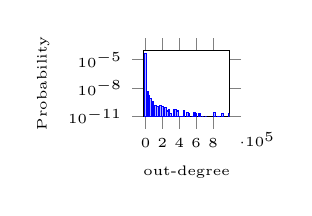
\begin{tikzpicture}
\begin{axis}[ymax=0.0001,ybar,ymode=log,bar width=19860.32,log origin=infty,xmin=-19860.32,ytick align=outside,enlargelimits=0,
width=.22\textwidth,
height=.20\textwidth,
ylabel=Probability,
xlabel=out-degree,
every x tick scale label/.style={at={(xticklabel cs:1)},anchor=south west},
  label style={font=\tiny},
tick label style={font=\tiny} ,
] 
\addplot  plot coordinates {
(0.0, 5.03431102238e-05)
(19860.32, 4.55404127627e-09)
(39720.64, 1.46577441888e-09)
(59580.96, 7.09840441847e-10)
(79441.28, 3.68748281479e-10)
(99301.6, 1.29061898518e-10)
(119161.92, 1.38280605555e-10)
(139022.24, 1.19843191481e-10)
(158882.56, 7.37496562958e-11)
(178742.88, 1.56718019629e-10)
(198603.2, 1.10624484444e-10)
(218463.52, 7.37496562958e-11)
(238323.84, 9.21870703698e-11)
(258184.16, 3.68748281479e-11)
(278044.48, 5.53122422219e-11)
(297904.8, 1.8437414074e-11)
(317765.12, 9.21870703698e-12)
(337625.44, 5.53122422219e-11)
(357485.76, 5.53122422219e-11)
(377346.08, 3.68748281479e-11)
(397206.4, 9.21870703698e-12)
(417066.72, 9.21870703698e-12)
(436927.04, 9.21870703698e-12)
(456787.36, 3.68748281479e-11)
(476647.68, 0.0)
(496508.0, 2.76561211109e-11)
(516368.32, 1.8437414074e-11)
(536228.64, 0.0)
(556088.96, 9.21870703698e-12)
(575949.28, 2.76561211109e-11)
(595809.6, 1.8437414074e-11)
(615669.92, 0.0)
(635530.24, 1.8437414074e-11)
(655390.56, 0.0)
(675250.88, 9.21870703698e-12)
(695111.2, 0.0)
(714971.52, 9.21870703698e-12)
(734831.84, 0.0)
(754692.16, 0.0)
(774552.48, 0.0)
(794412.8, 0.0)
(814273.12, 2.76561211109e-11)
(834133.44, 0.0)
(853993.76, 9.21870703698e-12)
(873854.08, 9.21870703698e-12)
(893714.4, 0.0)
(913574.72, 1.8437414074e-11)
(933435.04, 0.0)
(953295.36, 0.0)
(973155.68, 0.0)
(993016.0, 1.8437414074e-11)
};\end{axis}
\end{tikzpicture}
%\end{document}